\chapter{実験2 : 病理画像データセットを用いた実験}
\section{概要}
MNISTの実験から、提案したクエリ選考基準は、既存手法よりもCNNにとって識別率向上に寄与するサンプルを選択できていることが確認できた。
本章では、本研究で提案するシステムを用いて実際に病理画像データセットに対して行った実験について説明する。

\section{実験設定}
\subsection{データセットについて}
本実験では、Camelyon Grand Challenge\cite{Camelyon17}にて公開されたCamelyonデータセットを利用した。
Camelyonデータセットは1000枚のWSIからなり、乳癌のリンパ節転移を自動で検出する識別器を生成することを目的としたデータセットである\todo{図}。
各WSIは一枚あたり100,000×100,000ピクセルの大きさで、細胞組織を含む画像パッチは約10,000から400,000枚になる。
また、それら全ての画像パッチに対して癌か正常かの二値のラベルが付与されている。
ここでも、MNISTで行った実験と同様に各画像パッチのラベルは、クエリとして問い合わせない限り与えられない状況とする。


\subsection{実験の詳細}
Mnistの実験の際とは異なり、訓練用WSIに含まれる全ての画像パッチをラベルなしデータセット$\mathcal{U}$として利用した場合、その数は約6,000,000サンプルに登ってしまう。
このサンプルプールから、あるクエリ選考基準を最大化するサンプルを選択するのは計算コストの点から実用上困難である。
そこで、クエリ問い合わせ毎に利用可能な画像パッチ全体から一部をサンプリングすることで$\mathcal{U}_i$を作成し、
この中からモデル更新に寄与するサンプルを選択するようにする。各$\mathcal{U}_i$のサイズは50,000に設定した。

識別機に用いるCNNはGoogLeNetを採用した。他の一般画像認識で利用されるCNNのアーキテクチャの中でも比較的計量で、
医療画像解析ではしばしば用いられるモデルであることから選択した。\todo{引用と図}
少ないラベルで高精度を達成するために、ImageNetで学習済みのpretrained-modelを初期値として、転移学習によって学習を行う。

本実験でも、同一クエリ内での情報の重複を避けるためクラスタリングを行う。
第3章の予備実験から、クラスタリングに使用する特徴量はCompact Bilinear Poolingを用いたテクスチャ特徴量が有効だと推測される。
committeeサイズは10, k-meansのクラスター数$K$は1000、一度に選択するクエリ$\mathcal{Q}$のサイズは100に設定した。
Mnistでの実験のように各iterationでの学習回数を固定にせず、より現実的な状況に近づけるため、
与えられた比較的小さいバリデーションセットの性能が変化しなくなるまで学習を行う、という設定にした。

また、クラスターの代表サンプルから無作為にサンプリングされた100個のサンプルにラベルを付与して学習初期のラベルつきデータとして実験を開始した。
各クエリ問い合わせ毎に10000枚のテストデータに対する識別精度を計測し、ラベルを付与されたデータが10000に到達するまで実験を続けた。
実験ごとのばらつきを考慮し、同一の実験を3回行いその平均と標準偏差を計算した。

\section{実験結果}

\begin{figure}[tbp]
    \label{fig:mnist_acc_graph}
     \begin{center}
      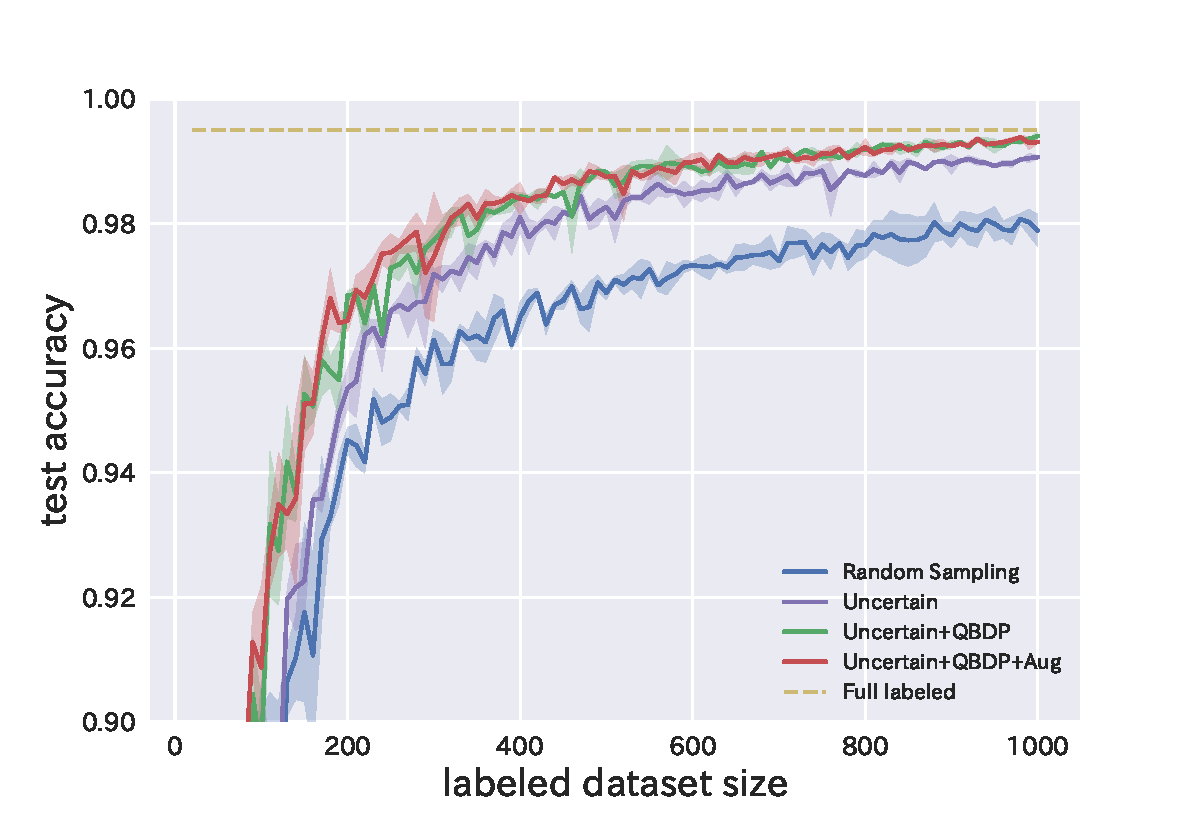
\includegraphics[width=10cm]{figures/mnist_acc_graph.pdf}
     \end{center}
    \caption{各手法を利用した場合のラベル付きサンプル数の増加に対するテスト精度の変化を示した図}
\end{figure}

\section{考察}
